% Author: Till Tantau
% Source: The PGF/TikZ manual
\documentclass[margin=2pt]{standalone}

% HdpH-RS: A Reliable Distributed Language

% Design
%% Language primitives
%% Fault tolerant scheduling protocol
%% Operational semantics
% Scheduler Validation
%% Promela abstraction
%% SPIN verification
% Implementation
%% Reliable scheduler
%% Fault tolerant communication
% Evaluation
%% 1400 cores on HPC
%% 256 cores with failure
%% Chaos monkey

\usepackage{tikz}
\usetikzlibrary{mindmap,backgrounds}
\begin{document}
\pagestyle{empty}
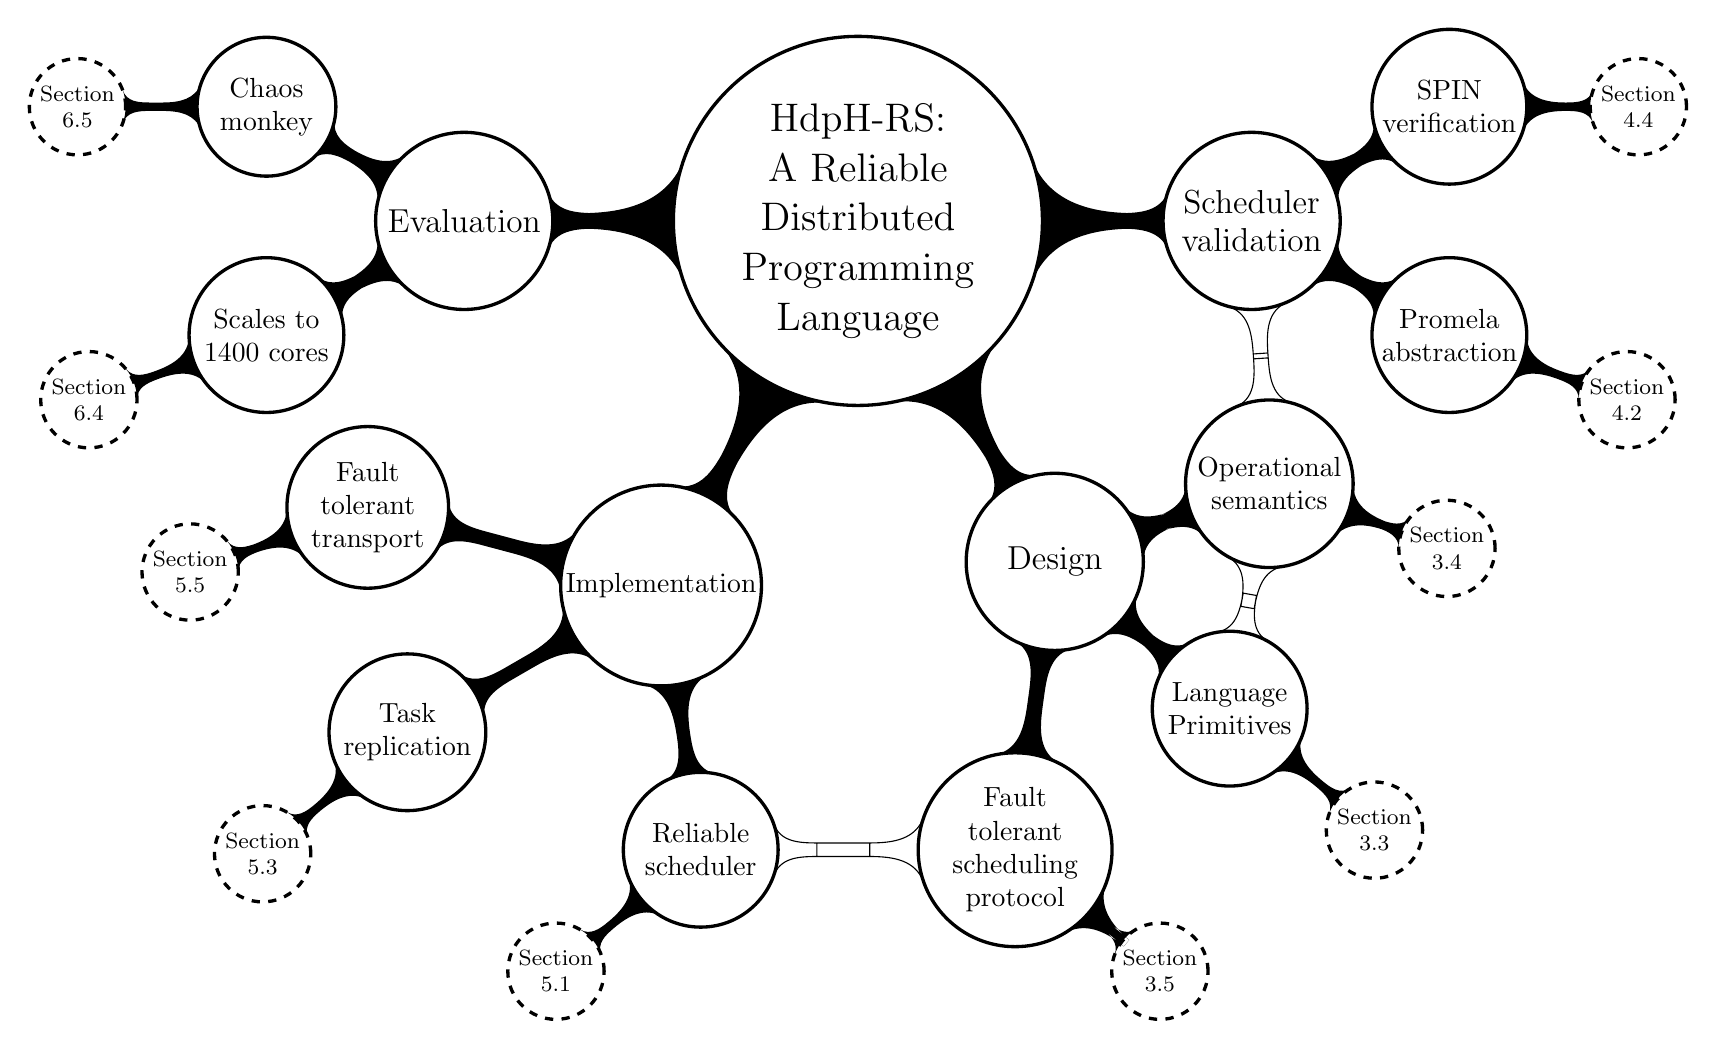
\begin{tikzpicture}[mindmap,concept=black,paper/.style={draw=gray,dashed}]
  \node[concept,fill=white,font=\Large] {HdpH-RS: A Reliable Distributed Programming Language}
  [clockwise from=0]
  child[concept] {
    node[concept,fill=white,font=\large] (validation) {Scheduler validation}
    [clockwise from=30]
    child { node[concept,fill=white,minimum size=5em,text
      width=5em,font=\normalsize] (spin) {SPIN verification}
      child[grow=0] { node[paper,concept,fill=white,font=\footnotesize] {Section \\ 4.4} }
    }
    child { node[concept,fill=white,minimum size=5em,text width=5em,font=\normalsize] (promela) {Promela abstraction}
      child[grow=-20] { node[paper,concept,fill=white,font=\footnotesize] {Section \\ 4.2} }
    }
  }
  child[concept] {
    node[concept,fill=white,font=\large] {Design}
    [clockwise from=20]
    child { node[concept,fill=white,minimum size=5em,text
      width=5.5em,font=\normalsize] (semantics) {Operational
        semantics}
      child[grow=-20] { node[paper,concept,fill=white,font=\footnotesize] {Section \\ 3.4} }
    }
    child { node[concept,fill=white,minimum size=5em,text
      width=5em,font=\normalsize] (primitives) {Language Primitives}
      child[grow=-40] { node[paper,concept,fill=white,font=\footnotesize] {Section \\ 3.3} }
    }
    child { node[concept,fill=white,minimum size=5em,text
      width=5em,yshift=-0.8cm,font=\normalsize] (protocol) {Fault
        tolerant scheduling protocol}
      child[grow=-40] { node[paper,concept,fill=white,font=\footnotesize] {Section \\ 3.5} }
    }
  }  
  child[concept] {
    node[concept,fill=white,minimum size=7em,text width=7em,font=\normalsize, yshift=-0.3cm] {Implementation}
    [clockwise from=-80]
    child { node[concept,fill=white,minimum size=5em,text
      width=5em,font=\normalsize, yshift=-0.5cm] (scheduler) {Reliable
        scheduler}
      child[grow=-140] { node[paper,concept,fill=white,font=\footnotesize] {Section \\ 5.1} }
    }
    child { node[concept,fill=white,minimum size=5em,text
      width=5em,font=\normalsize, xshift=-1cm] {Task replication}
      child[grow=-140] { node[paper,concept,fill=white,font=\footnotesize] {Section \\ 5.3} }
      }
    child { node[concept,fill=white,minimum size=4.5em,text
      width=4.5em,font=\normalsize, xshift=-1cm, yshift=0cm] {Fault
        tolerant transport}
      child[grow=-160] { node[paper,concept,fill=white,font=\footnotesize] {Section \\ 5.5} }
      }
  }
  child[concept] {
    node[concept,fill=white,font=\large] {Evaluation}
    [clockwise from=-150]
    child { node[concept,fill=white,minimum size=5em,text
      width=5em,font=\normalsize] {Scales to 1400 cores}
      child[grow=-160] { node[paper,concept,fill=white,font=\footnotesize] {Section \\ 6.4} }
    }
    child { node[concept,fill=white,font=\normalsize] {Chaos monkey}
      child[grow=-180] { node[paper,concept,fill=white,font=\footnotesize] {Section \\ 6.5} }
    }
  }
  ;

  \begin{pgfonlayer}{background}
    \draw [fill=black,circle connection bar]
    (protocol) edge (scheduler)
    (primitives) edge (semantics)
    (validation) edge (semantics);
  \end{pgfonlayer}

\end{tikzpicture}\end{document}

%%% Local Variables:
%%% mode: latex
%%% TeX-master: t
%%% End:
